\documentclass[IEEEtran,letterpaper,10pt,titlepage,fleqn,draftclsnofoot,onecolumn]{article}
%notitlepage vs titlepage
%fleqn left align

%\usepackage{nopageno} %no page numbers
\usepackage{indentfirst}
\usepackage{alltt}                                           
\usepackage{float}
\usepackage{color}
\usepackage{url}

\usepackage{graphicx}                                        
\usepackage{amssymb}                                         
\usepackage{amsmath}                                         
\usepackage{amsthm}                                          

\usepackage{balance}
%\usepackage[TABBOTCAP, tight]{subfigure}
\usepackage{enumitem}
\usepackage{pstricks, pst-node}
\usepackage{geometry}
\usepackage{hyperref}
\usepackage{textcomp}
\usepackage{listings}
%allows for code snipets

\geometry{textheight=9.5in, textwidth=7in} 

\newcommand{\cred}[1]{{\color{red}#1}} %think function call, changes text to red
\newcommand{\cblue}[1]{{\color{blue}#1}} %text to blue
\definecolor{dkgreen}{rgb}{0,0.6,0}
\definecolor{gray}{rgb}{0.5,0.5,0.5}
\definecolor{mauve}{rgb}{0.58,0,0.82}
\lstset{frame=tb,
  language=c,
  aboveskip=3mm,
  belowskip=3mm,
  showstringspaces=false,
  columns=flexible,
  basicstyle={\small\ttfamily},
  numbers=none,
  numberstyle=\tiny\color{gray},
  keywordstyle=\color{blue},
  commentstyle=\color{dkgreen},
  stringstyle=\color{mauve},
  breaklines=true,
  breakatwhitespace=true,
  tabsize=3
}

\def\name{Brandon Ellis, Jiayu Han, and Jack Neff}
\def\class{CS 461}
\def\assignment{Design Document}

%PDF Properties
\hypersetup{
  colorlinks = true,
  urlcolor = black,
  pdfauthor = {\name},
  pdfkeywords = {CS461 Senior Capstone Design Document},
  pdftitle = {\class \assignment},
  pdfsubject = {\class \assignment},
  pdfpagemode = UseNone
}

\begin{document}
%TitlePage
\begin{titlepage}
  \begin{center}
    \vspace{1cm}
    
    \huge
    \textbf{Green Smart Gardening System: Design Document}
    
    \vspace{1.5cm}
    
    \large
        \textbf{Brandon Ellis, Jiayu Han, and Jack Neff}
    
    \vspace{5cm}
    
    Abstract
    
    \normalsize
    This document discusses some core components that will make up our final product, a solar powered gardening device that provides the user with environmental data. There are three key pieces of functionality that this document will cover: Soil Moisture, Air Temperature \& Humidity, and Microcontrollers. The first two of these relate to environmental sensors that the chosen microcontroller will connect to. The last section covers the microcontroller itself. Each of these sections offer a description of the required task and go on to contrast different options to achieve these tasks.
    
    \vfill
    
    \large
        CS 461\\
        Fall Term\\
    \end{center}
\end{titlepage}

\section{Introduction}

This document will discuss core design aspects of our Green Smart Gardening System. It will detail nine different pieces of core functionality and note the member of our group assigned to it. The individual pieces will be discussed based on their hierarchy, which is shown in the section below. The pieces themselves are Soil Sensors, Air Sensors, Board Logic, Power, Wi-Fi, Database, Web Application, Displaying Data, and Packaging. 	These pieces will be discussed in terms of developing our device, a green energy powered garden monitoring system.

\section{Hierarchy}

\begin{figure}[H]
  \caption{Piece Hierarchy}
  \centering
  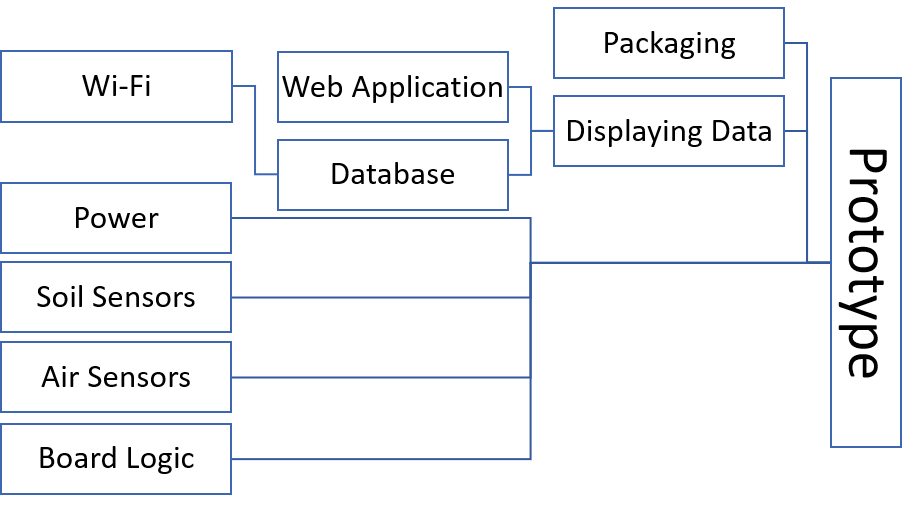
\includegraphics[width=0.5\textwidth]{hierarchy}
\end{figure}

\section{Design Pieces}
\subsection{Soil Sensors}
\subsubsection{Management: Brandon Ellis}

The first sensor related piece that will be covered is soil sensors. This section will cover two separate sensors, that together will achieve our devices soil requirements. These requirements being the measurement of soil moisture and soil pH. At this time, the two sensors that are being looked at to fill these roles are, respectively, the Phantom YoYo and the EZO pH Circuit. The process of integrating these sensors into our system will be the same for both. There will have to be a wired connection between each sensor and the board. There will need to be a software connection, so the board can easily communicate with the sensor. Finally, when this is all in place, the sensors will need to be tested.

\subsubsection{Hardware}

The first task in connecting the sensors to the board. For the YoYo, the required connections will be made through the sensor’s three pins: VCC, GND, and OUT. These three will support powering the YoYo and outputting measurements from it. Powering the sensor is fairly straightforward, with a wired connection simply needing to be made between the VCC and GND pins on the YoYo to their respective pins on the board. In order for the sensor to send information to the board, the last pin on the YoYo is used. The OUT pin is an analog output which can be connected to one of our board’s analog input pins. These three connections will be made through breadboard, in order to maximize the number of components our board can be interfaced with. 

\begin{figure}[H]
  \caption{YoYo Hookups}
  \centering
    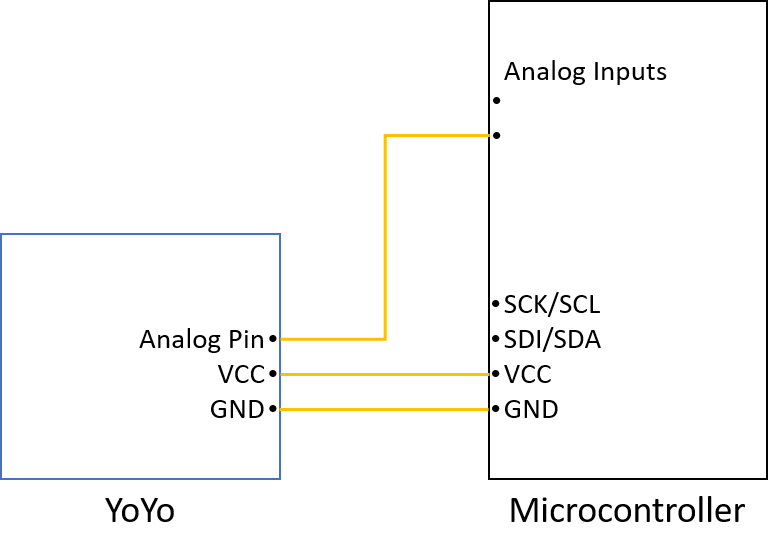
\includegraphics[width=0.5\textwidth]
  {yoyo_hookup}
\end{figure}

For the EZO pH Circuit, there are some slight differences in connections. Power will still be handled in the same fashion as the YoYo, with the sensor’s VCC and GND connecting to the VCC and GND power pins of the microcontroller. The main difference between these two sensors is how output is handled. The EZO, instead of a single analog pin, uses two pins. These two pins are TX/SDA and RX/SCL. What this provides is two different connection modes, UART and I2C, working through these pins. Our board has options for both types, though I2C will most likely be used as it is more versatile when working with multiple components. The final hookup for the EZO is its replaceable sensor. This is the portion of the device that physically goes into the soil. It is connected through two pins on the EZO that link via a breadboard to the soil sensor’s screw-in connection point.
\begin{figure}[H]
  \caption{EZO Hookups}
  \centering
    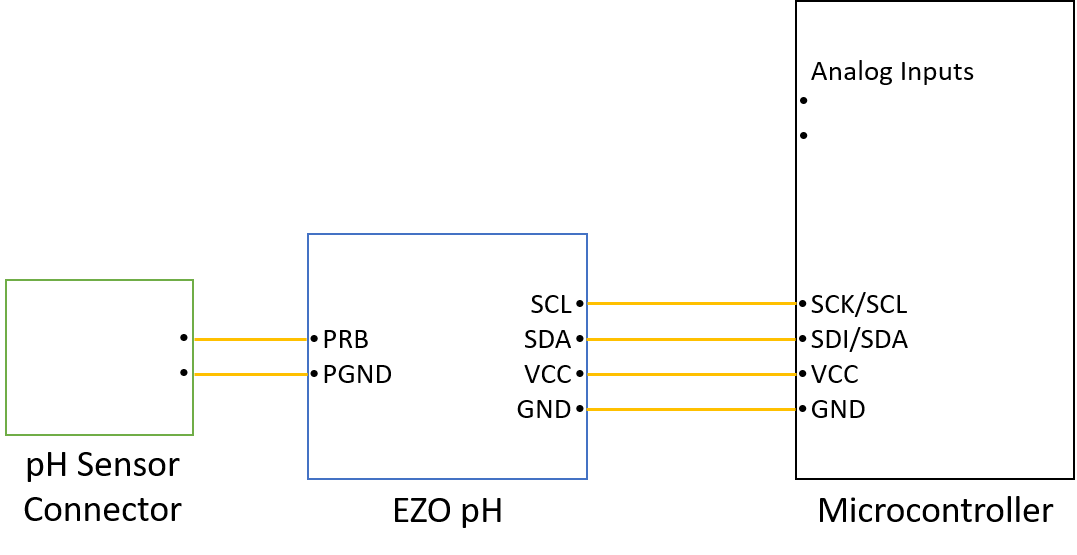
\includegraphics[width=0.5\textwidth]
  {ezo_hookup}
\end{figure}

\subsubsection{Software}

Once the hardware connections to these two sensors have been made, the board needs to understand how to communicate with it. For the YoYo, using analog methods, this a simple matter of assigning the pin internally on the microcontroller and using the read command. The EZO on the other hand, because of its I2C communication mode, will require a little more work. In order to communicate with this sensor, the board will have to note its address and then perform reading operations on it in a slightly more expanded manner than using a single command. Sample code is provided for the EZO on exactly how to make this communication. 

\subsubsection{Testing}

When these two steps have been completed, a physical connection between the sensors and board has been made and data is able to be transferred to the microcontroller. When other pieces of our device have been implemented, specifically saving data to an SD card and wireless connectivity, testing can then be done. The actual testing of these sensors will be done through the Oregon State Greenhouses to compare against a reliable and accurate source. 

\subsection{Air Sensor}
\subsubsection{Management: Brandon Ellis}

The second large sensor piece that will be covered is air sensors. In order to fulfill the required functionality for our air sensor, we need to measure air temperature and humidity. The component chosen to fill this role is the SparkFun Atmospheric Sensor Breakout BME280. The BME280 not only measures both relative humidity and temperature, but also notes the barometric pressure. To integrate this sensor with our system there will need to be a wired connection between the device. This will then allow communication from the sensor to our board, which will in turn allow us to test the validity of our data.

\subsubsection{Hardware}

The first step in this process is the physical connection of the BME280 to our board. In order to connect the two, the sensor requires power and a method of communication. To facilitate power, the BME280 has two pins that will need to be wired to the board. These are VCC and GND, to respectively provide 3.3V of power and a ground line. When these have been connected, there are then two forms of communication that the BME280 can utilize. In the above section, the EZO pH Circuit had two communication methods sent over the same pins. The BME280 differs by having two completely separate buses that each have their own method of communication, I2C and SPI. Though, like the EZO, the method of communication that we will be using is I2C, as it is the best method when working with multiple components connecting to a board. Connecting through I2C will entail connecting two pins, SDA and SCL, to their respective pins on our microcontroller.

\begin{figure}[H]
  \caption{BME280 Hookups}
  \centering
    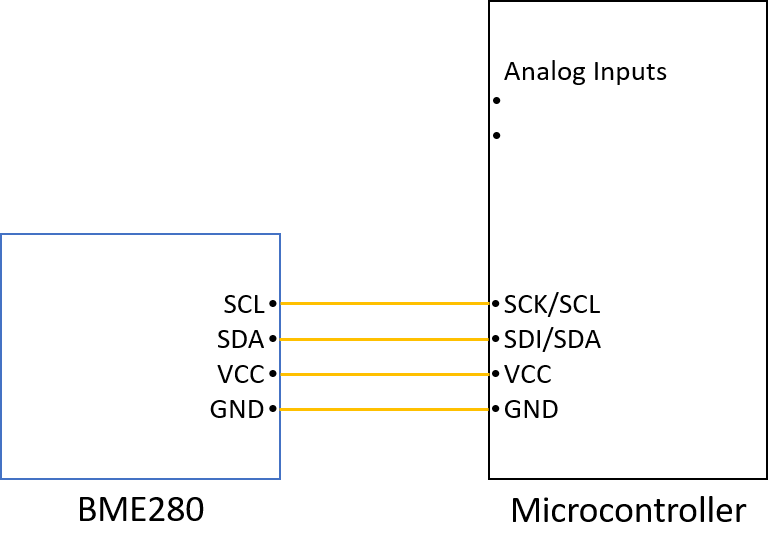
\includegraphics[width=0.5\textwidth]
  {bme280_hookup}
\end{figure}

\subsubsection{Software}

When first step is complete, a hardware connection has been created to our sensor. The microcontroller then needs to have software created to communicate with the sensor and retrieve data from it. Because of the method of communication being through I2C, the implementation of software for the BME280 will require noting the I2C address and dictating operations for the sensor. To do this, the BME280 provides several pieces of sample code and example configurations.

\subsubsection{Testing}

Finally, when the hardware and software connections have been created data can be outputted from the sensor to the board. At this time, assuming that functionality is in place to further output data wirelessly or to a SD card, testing can begin. Like the above soil sensors, testing will be done with the Oregon State Greenhouses in order to test the accuracy of our data points against theirs. 

\subsection{Power}
\subsubsection{Management: Jiayu Han}

For the power source section, there are some criteria we need to follow. First, Green Smart Gardening System needs to use renewable energy as the primary power source, it is supposed to use solar power as much as possible. Second, the device is supposed to run without any solar power for an entire week since Oregon rains so often during November to March. It will be hard to fully rely on the solar power during the wet season in Oregon. 

To reach the first criterion, the device needs to be powered by the solar power for most of the time. The micro-controller, Arduino MKR1000, has a great feature to achieve it. According to Arduino website [1], MKR1000 has two battery connectors, the USB power source and the Vin. The USB power source will be disconnected if there is appropriate power detected through Vin. The board has a 5V power supply voltage and a 3.3V operating voltage. By plugging the 5V solar panel through the Vin and the 3.7V Li-ION batteries through the USB, the board will always use the solar panel as the power source when it is available.  Based on the reviews on SparkFun [2], the solar panel will become undetectable once the voltage drops below 3.3V, and the Li-ION batteries will kick in from that.

\begin{figure}[H]
  \caption{MKR1000 Power[3]}
  \centering
    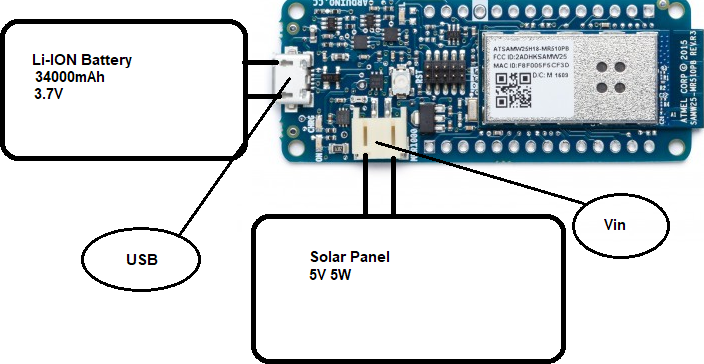
\includegraphics[width=0.5\textwidth]
  {power_graphic_1}
\end{figure}

As a backup plan for the power source, the solar module for Arduino [5] is also a great solution. It combines the solar panel and rechargeable batteries into one power source for the Arduino board. The module can handle two different inputs. The 3.7V to 7.0V one will be able to charge the battery, and the 3.7V to 6.0V one will be able to carry out the charge from the USB. Both solar panel and batteries are easy to change to the specific ones fit the device.

\begin{figure}[H]
  \caption{Solar Module[5]}
  \centering
    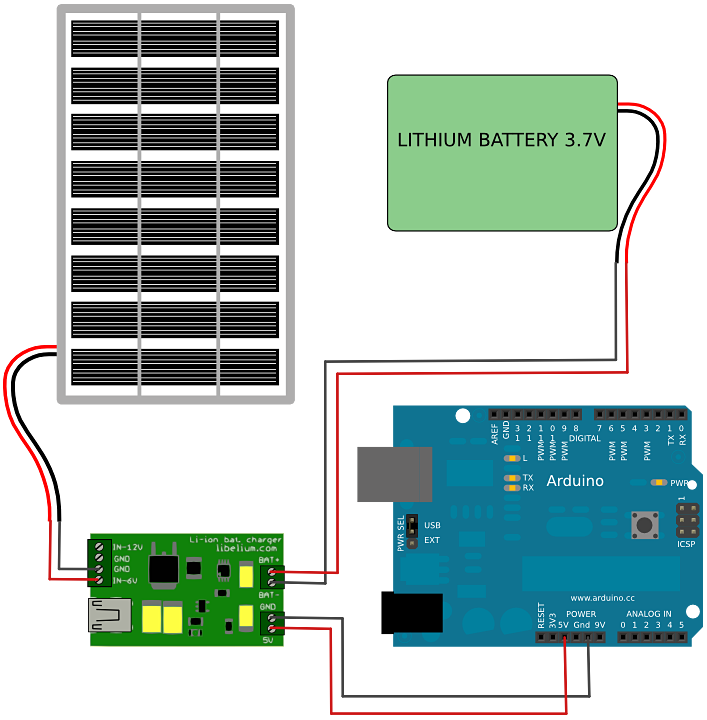
\includegraphics[width=0.5\textwidth]
  {power_graphic_2}
\end{figure}

To achieve the second criterion, the battery capacity needs to be at least 34000mAh. According to Arduino, the Wi-Fi module on MKR1000 absorbs roughly 100mA when connected to Wi-Fi with data transferring. The board consumption without Wi-Fi module initialized is 20mA. Based on the specs from the Technology Review document for the project, the preferred air temperature and humidity sensor and soil moisture sensor have a total of 21mA. Based on the equation from Arduino website, Battery Life = (Battery Capacity)/ (Maximum Current Consumption) * 0.7, we can get the equation for battery capacity, Battery Capacity = (Battery Life) *(Maximum Current Consumption)/0.7, which the battery capacity = (7*24h) * (141mA)/ 0.7 = 33840mAh.

\subsection{Wi-Fi}
\subsubsection{Management: Jiayu Han}

One of the biggest benefits of choosing Arduino MKR1000 as the micro-controller is that it comes with the ATSAMW25 Wi-Fi module on board, which makes it the ideal solution for designing IoT project. The on-board Wi-Fi module has up to 72Mbps with a great operating temperature range from -40°C to +85°C.

In order to get the Arduino MKR1000 connected to Wi-Fi, you will only need the MKR1000 with Arduino IDE. Before connecting the MKR1000 with the Wi-Fi, the MKR1000 needs to be already set up to connect to computer and able to upload custom sketch. After the MKR1000 is successfully connected, we will go to the Arduino WIFI 101 Shield repository on GitHub[6] to aquire the zipped Wi-Fi library. Then, we will open the Arduino IDE, find the “Include Library” in Sketch menu, and click “Add .ZIP Library” to add the repository. After these three steps, the MKR1000 is ready to connect to the Wi-Fi. We will need to include the WiFi101 library in the sketch and pick the Wi-Fi which it needs to connect to. 

\subsection{Board Logic}
\subsubsection{Management: Brandon Ellis}

Board logic handles the overarching software that will control and coordinate our device. While each of the sensors will have its own software associated with it, the purpose behind those pieces is heavily focused on communication and data retrieval. This section will detail some of the broad functionality that will be created as well as their associated testing.

The main pieces of functionality that will be discussed are data retrieval, outputting data, and scheduling. Out of these three, data retrieval is going to play the most off the software developed for each sensor. This piece of functionality will be responsible for querying those implemented functions and returning with the data. Once data has been retrieved, the data outputting portion will take over handling it. Retrieved data will be formatted and stored on an SD card. This will serve as a way to first back up the data. As our device is run off solar power and a battery, in the event of poor weather conditions for an extended period we need to be able to save the data in case transmitting would cause too much of a power draw. This way, when data is outputted it will be collected from the SD card to ensure it is backed up prior to transmission. The final piece of functionality that will be added is scheduling. Scheduling is the automated nature of our device to ensure that readings are taken in standard intervals. This addition will control when readings are taken from each sensor and when data this data will be transferred.  

Finally, this leaves how these pieces of functionality will be tested. There will be two main types of testing done on this software. The first will cover data retrieval and output, which is through unit testing. This will simply ensure that each of these individual pieces are operating correctly. The other type of testing that will be conducted is integration testing. This will be used to validate the scheduling portion, specifically this style of testing will aid in making sure that all of the individual pieces are able to work in tandem within our system.

\subsection{Database}
\subsubsection{Management: Jack Neff}

The storage and access of data is one of the most important aspects of our project, which is very data driven. Without the ability to consistently gather and store data, our application would be useless. This begs the question as to what database should we use, and what storage engine within that database? 

Database availability was the chief factor here. Each platform has a database software associated with it, so by selecting a platform one effectively is restricted to that platform’s database. We reasoned that users wouldn’t have much to do with the database. In fact, the less they have to do with it, the better. Therefore we picked our database solely based on our own needs and whether it met them. MySQL is one the three of us are all familiar with, and since it is supported by Google Cloud, we opted to go with it. [7]

We have more choices for the database storage engine. Our database has few outstanding requirements. Speed is not our top concern. Although we want to make sure our application is never sluggish, the nature of our application would allow us to voluntarily reduce data throughput in case of a slowdown, with minimal performance impact. For example, if we queried the database to graph environment data for a full year, we could leave out every other data point to reduce the workload by half, and still end up with a similar graph, provided our measurement interval is short enough. Additionally, In order to implement our preferred structure, foreign key support will be required, for cross-table references, as well as transaction support for data simplification possibly the computation of metrics. This led us to select InnoDB as our storage engine, because it supports foreign keys and transactions, is very fast, and we have all used it before. Also, InnoDB supports multi-view concurrency control (MVCC), which means we can all work on the database at the same time with no issues.[8]

A final design consideration regarding the database is what should be stored, and in what form? Our data will consist mostly of environmental measurements associated with a timestamp. For example, one database column could be Temp and another could be Time. This would allow us to graph the temperature over time. To simplify data analysis and display, we will design the input to come through in “packets.” We are measuring a lot of environmental factors (temperature, humidity, soil moisture, etc.), and if they each had their own timestamp, things would get very messy. Therefore, we want these packets to hold one measurement of each environmental variable, coupled with a timestamp that corresponds to all those measurements. These packets will be easily graphed and will be highly comparable because of their common timestamps, which will make generating views easier.

\subsection{Web Application}
\subsubsection{Management: Jack Neff}

Server stack implementation is an important software design decision for us. We refer to this design aspect as the server platform. The question is, what platform should we select to store and maintain our application and all its data? Users will be dependent on this platform to support their data needs, and to form the operational infrastructure of the Gardening System. Primarily we want to direct this design based on scalability and reliability, with a secondary concern for ease of use by the user. 

One design decision involving the server stack is what operating system we want it to be usable on. Several popular server platform stacks such as WAMP are windows only, while others are specifically designed for Linux, and still others work with any OS. In the interest of reaching the largest possibly client base, we wanted to use a server stack that was supported on all operating systems. This is one of the design points that led us to select Google Cloud Platform as our web server: it isn’t platform specific.

Another factor is scalability. As a group we have experience of hosting http servers on a local virtual machine, only to have performance suffer when data operation and data storage volumes became too large for it to handle. The Google Cloud Platform is supported on hearty and fast infrastructure, the same which supports google searches, or playback of YouTube videos. It is a tried and true resource capable of handling lots of computing, which we may need if we ever adapt our design full scale. Our prototype will be a small system consisting of one of a few plants, but the large scale implementation of a vineyard or orchard (or multiple) would significantly increase data throughput and calculations done in analysis. 

One fairly obvious design choice was what language to use to implement the web application. The language needs to be able to interface between database and web browser, and should preferable be simple, and a language we the developers are already familiar with. We selected PHP because it is supported by all server platforms, and is known for being one of the easiest if not the easiest language for accessing databases. It also helps that all three of us have experience programming in PHP, and querying databases in PHP. 

Other, lesser factors included reliability and ease of use by the developers. Reliability is not an emphasis here simply because most server platform stacks are pretty reliable. Google Cloud Platform though, especially, is known to be very reliable, since it is based on Google’s famous infrastructure. Ease of use was a concern entirely our own, and is important because selecting an easy-to-use application saves time and effort that could have been spent debugging or learning to use the software. Known for being easy to use and for having a large body of community support online, the Cloud Platform satisfies this requirement well. 

\subsection{Displaying Data}
\subsubsection{Management: Jack Neff}

Data display is the key to bringing information to the user in a way that is easy to understand and can inform their agricultural decisions. Data displays should be easy to understand, and be viewable on the web-based user interface. Users should be able to easily construct their own graphs based on available data. In addition, some graphs should be automatically generated from data in the database. This part of our design is completely geared toward the user. We want to make the data we collect very understandable, even by someone without a lot of math, computer, or agricultural experience. Also, we want to give the user relevant information, rather than just bombarding them with numbers and timestamps. Finally, we want the data to look good, and dynamically create graphs and views without causing any slowdown.

To fulfill cosmetic requirements, we selected D3js as our API for data display. This is a JavaScript library that provides lots interesting data display functionality. In addition, because it is a JavaScript library and not a program itself, we expect it will be fast and lightweight. [9]

When the user logs into the web application, they should have the most valuable information distilled for them on the main page. Although at first in our design we flirted with trying to implement low-level machine learning, we have now realized there won’t be enough time, so we will be doing independent research into plant growth to find out what types of plants are healthy in what environments. Using these known benchmarks, we will provide users with information about their system’s environment, and how this information relates to the ideal environment conditions for a plant. An early design idea is to have a colored bar or a circle for each environmental variable plainly visible on the application front page. If the variable is within acceptable bounds, the graph element would be green, and red if not. By clicking on that element, a user could view a graph of that element by itself over time, and analyze why it is out of the required range.

One interesting design consideration is how much freedom to allow the user to have when graphing their own data. Because users of this product may not be very computer-savvy, the users’ ability to make their own graphs should be limited to a few preset options, to avoid presenting them with an overwhelming array of choices. Variables should be graphable against one another, as well as against time, and there should be a wide number of graphical options for each type of graph. D3js specializes in radial displays and maps, and since we won’t be needing maps, we will likely design a number of radial displays. Users should be able to save their graphs and mount them on the front page of the web app if they like. 

One of the keys to an enjoyable user experience is speed and responsiveness of an app. We want the user to see graphs as soon as they log in, but if these dynamic graphs hurt performance, that is unacceptable. We will implement some kind of contingency against this, so instance, if the application detects that the front page of the app is loading slowly, it should cut the number of data points in half by selecting every other one, and then reload the page. User experience needs to be the absolute focus of this design element. There is no utility in showing off data or graphs unless the user wants to view them and is not put off by long loading times.

\subsection{Packaging}
\subsubsection{Management: Jiayu Han}

Our vision of the device will be stored in a package. The micro-controller and the batteries along with most of the cables will be stored inside of the case in order to protect them from damaging. Outside of the package will only have the solar panel, the soil moisture sensor and the air temperature \& humidity sensor to collect the energy to power up the device and the data for analyzation. In order to make the device package firm with high pressure resistance, cylindrical package will be the best option. It will easily hold its shape to protect the device inside from sticking into the soil. The solar panel will be set at the top of the package so that it could produce solar power at its maximum efficient. The air temperature \& humidity sensor will extend from the top of the side so that the temperature and humidity will have a lower chance of appearing errors because of the ground temperature and humidity. The soil moisture sensor will come out from the bottom of the package in order to get to the similar depth as the root of the plants to collect more precise data.

Based on the purpose of the Green Smart Gardening System, the device needs to be used outdoor and waterproof. Since the Green Smart Gardening System is meant to be an IoT device, we need to avoid any metal case to ensure that we can get the best Wi-Fi connection. Because the device is meant to work outdoor in Oregon, where has a long wet-season, we need to keep the package fully sealed up to prevent the water and other stuffs in the soil from corroding and short circuit. Since the temperature in Oregon could range from -10°C to 40°C+ during the year, the material of the case need to sustain both low and high temperature. The lunch box like plastic material could be a great choice. 

\clearpage

\section{References}
[1] "Arduino MKR1000 WIFI", Arduino, 2017. [Online]. Available: https://store.arduino.cc/usa/arduino-mkr1000. [Accessed: 30- Nov- 2017].

\vspace{1mm}

[2]"Arduino MKR1000 (with Headers) - DEV-14393 - SparkFun Electronics", Sparkfun.com, 2017. [Online]. Available: https://www.sparkfun.com/products/14393. [Accessed: 30- Nov- 2017].

\vspace{1mm}

[3]Arduino, Arduino MKR1000 WIFI. 2017.

\vspace{1mm}

[4]"Solar Module for Arduino", Cooking-hacks.com, 2017. [Online]. Available: https://www.cooking-hacks.com/documentation/tutorials/arduino-solar/. [Accessed: 30- Nov- 2017].

\vspace{1mm}

[5]Cooking Hacks, Solar Powered Arduino. 2017.

\vspace{1mm}

[6]"arduino-libraries/WiFi101", GitHub, 2017. [Online]. Available: https://github.com/arduino-libraries/WiFi101. [Accessed: 30- Nov- 2017].

\vspace{1mm}

[7]S. Hull, "MySQL face-off: MySQL or MariaDB?", InfoWorld, 2017. [Online]. Available: https://www.infoworld.com/article/2611812/mysql/mysql-face-off--mysql-or-mariadb-.html. [Accessed: 30- Nov- 2017].

\vspace{1mm}

[8]"MySQL :: MySQL NDB Cluster 7.5 :: 3.5.1 Differences Between the NDB and InnoDB Storage Engines", Dev.mysql.com, 2017. [Online]. Available: https://dev.mysql.com/doc/mysql-cluster-excerpt/5.7/en/mysql-cluster-ndb-innodb-engines.html. [Accessed: 30- Nov- 2017].

\vspace{1mm}

[9]M. Bostock, "D3.js - Data-Driven Documents", D3js.org, 2017. [Online]. Available: https://d3js.org. [Accessed: 30- Nov- 2017].

\end{document}